\section{trigonometric functions, radians}
%%%%%%%%%%%
%%%%%%%%%%%

In Chapter~\ref{sec:funzioni_trigonometriche}, we defined the functions $\sin$
and $\cos\colon \RR\to \RR$ with period $\tau>0$ (arbitrary) such that the
function $\phi\colon \RR\to\RR^2$, $\phi(t)=(\cos t, \sin t)$ traverses, with
uniform circular motion, in a counterclockwise direction, the unit circle
$\ENCLOSE{(x,y)\in \RR^2\colon x^2+y^2=1}$. This function indeed describes a
uniform circular motion as it traverses congruent arcs in equal times.
\mynote{Two geometric figures are \emph{congruent} if there is an isometry that maps one onto the other. Two arcs are congruent if they have the same length and the same radius, but it is not necessary to introduce the concept of \emph{arc length} to discuss congruence.}

We now wish to show that it is possible to choose the constant $\tau$ such that
the path described by $\phi$ traverses the circle with unit \emph{velocity}.
\mynote{Recall that $\tau$ is the period of the functions $\phi$, $\cos$, and $\sin$}%
If I follow the point $f(t)$ starting from the instant $t=0$ for a short time
$\Delta t\neq 0$, I observe that the point moves between $f(0) = (1,0)$ and
$f(\Delta t) = (\cos \Delta t, \sin \Delta t)$.
\mynote{The notation $\Delta t$ indicates any positive number. We use this notation because this number represents a difference ($\Delta$ is a Greek letter $D$) of times that are close to each other.}%
Intuitively, when $t=0$, the point $f(t)$ moves vertically, upwards. The
distance traveled $\Delta s$ will therefore be approximately equal to the change
in the $y$ coordinate: $\Delta y = \sin \Delta t$.
\mynote{Recall that $\sin 0 = 0$}
Thus, the velocity will be equal to the vertical component of the velocity and
will be, intuitively, the limit of $\frac{\Delta y}{\Delta t}$, that is,
\mynote{We will soon see that this limit is the \emph{derivative} of the function $f$ at the point $t=0$.}
\[
\lim_{\Delta t\to 0} \frac{\sin(\Delta t)}{\Delta t}.  
\]

From a formal standpoint, it is not entirely obvious that this limit exists. We
will demonstrate it using a method very similar to the one used to define the
constant $e$ of Napier. Just as the real exponential $x\mapsto a^x$ is an
isomorphism between the additive group of $\RR$ and the multiplicative group of
$\RR^+$, so the function $\phi(t) = (\cos(t), \sin(t))$ turns out to be an
isomorphism between the additive group $\RR$ and the group of plane rotations,
which can be represented by the set $U$ of unit complex numbers. We have already
seen that for the point moving with the law $x\mapsto a^x$ to have velocity $1$
at $x=0$, one must set $a=e$, the base of natural logarithms. Similarly, we will
now see that for the velocity of the point $t\mapsto \phi(t)$ to also be
unitary, we must have $\tau = 2\pi$. By combining the two isomorphisms $e^t$ and
$\phi(t)$, we will be able to define, as we will soon see, an isomorphism
between the additive group $\CC$ and the multiplicative group
$\CC\setminus\ENCLOSE 0$. What is obtained is the complex exponential $z\mapsto
e^z$. The velocity of $\phi(t)$ indeed represents the derivative of this complex
function at the point $1$ in the direction of the imaginary axis, just as the
derivative of the real exponential function is the derivative in the real
direction. Thus, it is inferred how the fundamental constants $e$ and $\pi$ are
related by the condition that the complex exponential function is differentiable
in the complex sense and has a complex derivative equal to $1$.

\subsection{the number $\pi$}

In this chapter, we must work with the functions $\sin$, $\cos$, and
$\tg=\frac{\sin }{\cos}$ introduced in
Chapter~\ref{sec:funzioni_trigonometriche}. These functions have been defined
with a period $\tau>0$ fixed arbitrarily starting from the function $\phi$
defined by Theorem~\ref{th:omomorfismo_U}. We will write $\phi_\tau$,
$\sin_\tau$, and $\cos_\tau$ when it is useful to highlight the dependence on
$\tau$. In this chapter, we will define the number $\pi$, and at that point, we
will always choose $\tau=2\pi$ as the measure of the full angle.

If we choose two different measures $\tau$ and $\sigma$ for the full angle, the
relationship between the two functions is simply:
\begin{equation}\label{cambio_angolo}
  \phi_\tau (\tau t) = \phi_1(t) = \phi_\sigma(\sigma t), 
\end{equation}
since $\phi_\tau(\tau t)$ satisfies the properties that uniquely define $\phi_1$
based on Theorem~\ref{th:omomorfismo_U}.

\begin{theorem}
\label{teo_limite_pi}
For every $x\in \RR$ with $0<x \le \frac \tau 2$, the sequence
\[
    a_n = n \sin_\tau \frac x n
\]
converges to a finite, positive limit.
\end{theorem}
%
\begin{proof}
We will make use of the function $\tg x= \frac{\sin x}{\cos x}$. We will use the
addition formulas:
\begin{align*}
 \sin(x+y) &= \sin x\cos y + \cos x \sin y,\\
 \cos(x+y) &= \cos x \cos y - \sin x \sin y  
\end{align*}
from which, by taking the ratio and dividing the numerator and denominator by
$\cos x \cos y$, we obtain:
\[
  \tg(x+y) = \frac{\tg x + \tg y}{1-\tg x \tg y}.
\]
We will also use the fact that on the interval $\closeinterval{0}{\frac \tau 4}$
\mynote{recall that $\tau$ is the (arbitrarily chosen) period of the functions
$\sin$ and $\cos$} the functions $\sin$ and $\cos$ have values between $0$ and
$1$. These properties are guaranteed by
Theorem~\ref{th:proprieta_trigonometriche}. The function $\tg x$ in turn is
defined if $0\le x < \frac \tau 4$ (since $\cos \frac \tau 4=$, the tangent is
not defined for $x=\frac \tau 4$).

\emph{Step 1:} we want to prove that if $n\in \NN$ and $t>0$, then
\begin{equation}\label{eq:4813509}
  nt <\frac \tau 4
  \implies
  n\sin t\le \tg nt.
\end{equation}
We prove it by induction. If $n=0$, it is obvious. Assuming \eqref{eq:4813509}
is true for a certain $n$, we now want to prove that if $(n+1)t < \frac \tau 4$,
then $(n+1)\sin t \le \tg (n+1)t$. Observe that if $(n+1)t<\frac \tau 4$, then
$nt < \frac \tau 4$, and the functions $\sin,\cos$, and $\tg$ are all positive
at the points $t$, $nt$, and $(n+1)t$. Thus, we have:
\begin{align*}
\tg (n+1) t 
  &= \frac{\tg nt + \tg t}{1-\tg nt \tg t}
  \ge \tg nt + \tg t \\
  &\ge n\sin t + \tg t \qquad\text{[by \eqref{eq:4813509}]}\\
  &\ge n\sin t + \sin t
  =(n+1)\sin t. 
\end{align*}

\emph{Step 2:} we prove that if $n\ge 2$, then $a_{n+1} \ge a_n$. To apply \eqref{eq:4813509}, we need $nt < \frac \tau 4$, i.e., $\frac x {n+1}< \frac \tau 4$, which is true since $x\le \frac {\tau} 2$ and $n\ge 2$. Thus, setting $t = \frac{x}{n(n+1)}$, we have:
\begin{align*}
  a_n &= n \sin\frac{x}{n+1} 
    = n \sin (n+1)t
    = n \sin nt \cos t + n \sin t \cos nt\\
    &\le n \sin nt \cos t + \tg nt \cos nt
    \qquad\text{[by \eqref{eq:4813509}]}\\
    &\le n \sin nt + \sin nt
    = (n+1) \sin nt = (n+1) \sin \frac x n.
\end{align*}

\emph{Step 3:} the sequence $a_{3n}$ is bounded. Indeed, we have
\begin{align*}
 a_{3n} = 3n \sin \frac x {3n} 
 \le 3\tg \frac x 3
\end{align*}
where we could apply~\eqref{eq:4813509} since $\frac x 3 < \frac{\tau }{2}$,
given $x\le \frac {\tau} 2$.

\emph{Step 4: conclusion.} By Step 2, the sequence $a_{n+1}$ is increasing, so by Theorem~\ref{th:limite_successione_monotona}, the sequence has a limit $a_n\to \ell$ as $n\to +\infty$. Since $a_n \ge a_2$ for every $n\ge 2$, we have $\ell \ge a_2 >0$. And, by Step 3, it cannot be $\ell=+\infty$, otherwise $a_{3n}$ would not be bounded.
\end{proof}

We provide a geometric interpretation of the previous result. We want to
calculate the length of an arc of measure $x$ on the unit circle. We divide the
arc into $n$ equal parts and consider the polygonal line formed by the chords on
the $n$ angles of measure $\frac {x} n$. In general, the chord on the angle
$\alpha$ of a circle of radius $r$ measures $2r \sin \frac \alpha 2$. Thus, the
polygonal line constructed on the arc $x$ measures $n\sin\frac{x}{2n}$. We would
therefore like to define $\pi$ as the limit of this sequence.

\begin{definition}[$\pi$ fundamental constant of trigonometry]%
  \label{def:pi}%
We define
\[
 \pi 
  \defeq \lim_{n\to +\infty} n\cdot \sin_\tau \frac \tau {2n}.
\]
where $\sin_\tau$ is the $\sin$ function constructed in
Theorem~\ref{def:sin_cos} with period $\tau$. Since $\sin_\tau \tau x =
\sin_\sigma \sigma x$, the limit does not depend on the choice of $\tau$. This
limit exists and is finite and positive by Theorem~\ref{teo_limite_pi}.
\end{definition}

Choosing $\tau = 360$, we find $a_4 = 4 \sin_\tau \frac{180}{4} = 2 \sqrt 2 >
2.8$, from which, by the monotonicity property of $a_n$, we find $\pi > 2.8$.
Observing that $a_{2^n} = 2^n \sin_\tau \frac{45}{2^{n-2}}\le 4 \tg_\tau 45 =
4$, we obtain $\pi<4$. We will find much more refined methods to determine the
approximate values of $\pi$, see for example Exercise~\ref{ex:cifre_pi} and
Table~\ref{tab:cifre_pi}.

\begin{theorem}[remarkable limit $\sin$]
  \label{th:limite_notevole_sin}%
For every $x\in\RR$, $x\neq 0$, we have 
\[
\lim_{x\to 0}\frac{\sin_{\tau} x}{x}
= \frac{2\pi}{\tau}.
\]
In particular, if we choose $\tau = 2\pi$, we have the remarkable limit:
\begin{equation}\label{eq:limite_notevole_sin}
 \lim_{x\to 0} \frac{\sin x}{x} = 1.
\end{equation}
\end{theorem}
%
\begin{proof}
First, we show that
\begin{equation}\label{eq:771743}
   \lim_{t\to+\infty} t \sin_\tau \frac{\tau}{2t} = \pi.
\end{equation}
Indeed,
\begin{equation}\label{eq:4961077}
  \frac{\lfloor t \rfloor}{\lceil t \rceil} \cdot \lceil t \rceil \sin_\tau \frac{\tau}{2\lceil t \rceil}
  \le \lfloor t \rfloor \sin_\tau \frac{\tau}{2\lceil t \rceil}
  \le t \sin_\tau \frac{\tau}{2t} 
  \le \lceil t \rceil \sin_\tau \frac{\tau}{2\lfloor t \rfloor}
  \le \frac{\lceil t \rceil}{\lfloor t \rfloor} \cdot \lfloor t \rfloor \sin_\tau \frac{\tau}{2\lfloor t \rfloor}
\end{equation}
and since 
\[
  \frac{\lfloor t \rfloor}{\lceil t \rceil}\to 1, \qquad
  \frac{\lceil t \rceil}{\lfloor t \rfloor}\to 1
\]
by the definition of $\pi$, both extremes of the chain of
inequalities~\eqref{eq:4961077} tend to $\pi$, and thus by the squeeze theorem,
we obtain the desired limit~\eqref{eq:771743}. With the change of variable
$x=\frac 1 t$, we obtain the limit~\eqref{eq:limite_notevole_sin} when $x\to
0^+$. The complete limit for $x\to 0$ is obtained by symmetry.
\end{proof}

From now on, we will choose $\tau=2\pi$ as the period of the trigonometric
functions. And from now on, it will be understood that $\sin = \sin_{2\pi}$,
$\cos = \cos_{2\pi}$. We will thus have the remarkable limit
\[
   \lim_{x\to 0} \frac{\sin x}{x} = 1.  
\]

When we introduce derivatives, we will also observe that this choice of period
$\tau=2\pi$ ensures that the point with coordinates $(\cos t,\sin t)$ moves with
unit velocity along the unit circle. Thus, this point traverses an arc of length
$t$ in time $t$. In particular, in one period $\tau=2\pi$, the point traverses
the entire circle, and thus it results that $2\pi$ is the length of the unit
circle (i.e., $2\pi r$ is the length of the circle of radius $r$). At time
$t=1$, the point $(\cos t,\sin t)$ identifies an angle called a \emph{radian}
because it corresponds to an arc of length equal to the radius (unitary). Thus,
the \emph{radian} is the natural unit of measure for measuring angles, and the
functions $\sin$ and $\cos$ will henceforth be fixed with this unit of measure.

\newsavebox{\qrfigtrigo}\sbox{\qrfigtrigo}{\myurlhere{figtrigo}{trigonometric functions}}%
\begin{figure}
  \centering%
  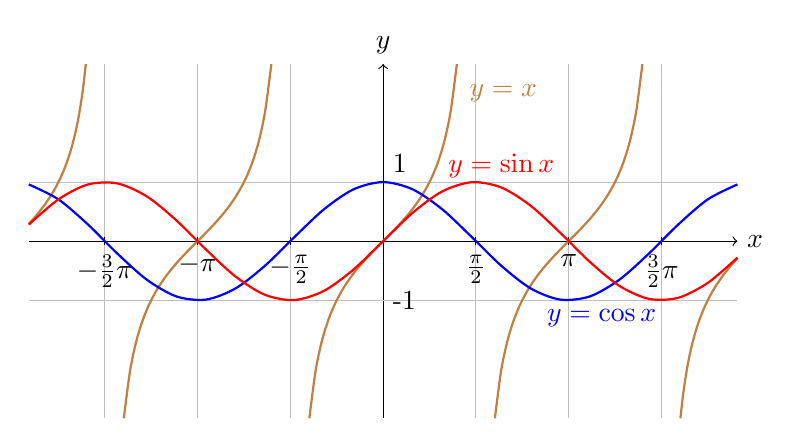
\begin{tikzpicture}[scale=0.75]
  \draw[->] (-6,0) -- (6,0) node[right] {$x$};
  \draw[->] (0,-3) -- (0,3) node[above] {$y$};
  \foreach \x/\xtext in
    {{pi/2}/{\frac \pi 2}, {pi}/{\pi}, {3*pi/2}/{\frac{3}{2}\pi},
    {-pi/2}/{-\frac \pi 2}, {-pi}/{-\pi}, {-3*pi/2}/{-\frac{3}{2}\pi}} {
    \draw[shift={(\x,0)},lightgray] (0,-3) -- (0,3);
    \draw[shift={(\x,0)}] (0pt,2pt) -- (0pt,-2pt) node[below] {$\xtext$};
  }
  \foreach \y in {1, -1} {
    \draw[shift={(0,\y)},lightgray] (-6,0) -- (6,0);
  }
  \draw (0,1) node [above right] {1};
  \draw (0,-1) node [right] {-1};
  \draw[domain=-rad(atan(3)):rad(atan(3)),smooth,variable=\x,brown,thick] plot ({\x},{tan(deg(\x))});
  \draw[domain=pi-rad(atan(3)):pi+rad(atan(3)),smooth,variable=\x,brown,thick] plot ({\x},{tan(deg(\x))});
  \draw[domain=-pi-rad(atan(3)):-pi+rad(atan(3)),smooth,variable=\x,brown,thick] plot ({\x},{tan(deg(\x))});
  \draw[domain=-6:-2*pi+rad(atan(3)),smooth,variable=\x,brown,thick] plot ({\x},{tan(deg(\x))});
  \draw[domain=2*pi-rad(atan(3)):6,smooth,variable=\x,brown,thick] plot ({\x},{tan(deg(\x))});
  \draw[domain=-6:6,smooth,variable=\x,blue,thick] plot ({\x},{cos(deg(\x))});
  \draw[domain=-6:6,smooth,variable=\x,red,thick] plot ({\x},{sin(deg(\x))});
  \draw (3.7,-1) node[blue,below] {$y=\cos x$};
  \draw (2,0.9)  node[red,above] {$y=\sin x$};
  \draw (1.3,2.5) node[brown,right] {$y=\tg x$};
  \end{tikzpicture}
  \caption{%
  The graphs of the functions $\sin$, $\cos$, and $\tg$.
  \ifwidemargin\\\\\fi%
  \usebox{\qrfigtrigo}}
\end{figure}

\subsection{inverse trigonometric functions}

The function $\sin\colon[-\pi/2,\pi/2]\to [-1,1]$ is strictly increasing and
bijective. Thus, by restricting the domain to the interval $[-\pi/2, \pi/2]$ and
the codomain to the interval $[-1,1]$, the function is invertible. The inverse
function
\[
  \arcsin\colon[-1,1]\to [-\pi/2, \pi/2]
\]
is called the \emph{arc sine}. It is a continuous function by
Theorem~\ref{th:monotona_continua} of continuity of monotone functions.

By definition of the inverse function, we have
\[
  \arcsin(\sin x) = x, \qquad \forall x \in [-\pi/2, \pi/2]
\]
and
\[
  \sin(\arcsin x) = x, \qquad \forall x \in [-1, 1].
\]

The function $\cos \colon[0,\pi] \to [-1,1]$ is strictly decreasing and
bijective. The inverse function
\[
  \arccos\colon[-1,1] \to [0,\pi]
\]
is called the \emph{arc cosine}. It is also continuous due to its monotonicity
properties. By definition, we have
\[
  \arccos(\cos x) = x, \qquad \forall x \in [0,\pi]
\]
and
\[
    \cos(\arccos x) = x, \qquad \forall x \in [-1,1].
\]

The function
\index{tangent!trigonometric function}
\mymargin{$\tg x$}%
\index{$\tg x$}
\[
\tg x = \frac{\sin x}{\cos x}
\]
is defined when $\cos x\neq 0$, i.e.,
\[
  \tg \colon \RR \setminus\ENCLOSE{\frac \pi 2+ k\pi\colon k\in \ZZ} \to \RR.
\]
If we restrict the function to the interval $\enclose{-\pi/2, \pi/2}$, we can
easily observe that the function $\tg\colon(-\pi/2,\pi/2)\to \RR$ is strictly
increasing. Moreover, if $a_n \to \pi/2$, $a_n<\pi/2$, we have $\cos(a_n)\to 0$
(by continuity of the cosine) and $\sin(a_n)\to 1$, thus $\tg a_n\to +\infty$.
Similarly, for $a_n \to -\pi/2$, we find $\tg a_n \to -\infty$. Thus, by the
intermediate value theorem, we can assert that the function
$\tg\colon(-\pi/2,\pi/2)\to \RR$ is surjective. It is therefore invertible, and
the inverse function
\[
  \arctg \colon \RR \to (-\pi/2,\pi/2)
\]
is called the \emph{arc tangent}. By definition, we have
\[
  \arctg \tg x = x, \qquad \forall x \in (-\pi/2, \pi/2)
\]
and
\[
  \tg\arctg x = x, \qquad \forall x \in \RR.
\]

Thanks to Theorem~\ref{th:monotona_continua}, since these functions are monotone
and bijective, we can assert that the functions $\arcsin$, $\arccos$, and
$\arctg$ are all continuous functions.

\begin{exercise}[mysterious functions]
  Draw the graph of the following functions
  \[
    f(x) = \arcsin \sin x, \qquad 
    g(x) = \arccos \cos x, \qquad 
    h(x) = \arctg \tg x.
  \]
  Observe that:
  \begin{enumerate} 
    \item $f$ and $g$ are defined on all of $\RR$, while $h$ is defined on $\RR\setminus\ENCLOSE{\frac{\pi}2+k\pi\colon k\in \ZZ}$;
    \item $f$ and $h$ have values in $\closeinterval{-\frac \pi 2}{\frac \pi 2}$, while $g$ has values in $\closeinterval{0}{\pi}$;
    \item $f$ and $g$ have period $2\pi$, $h$ has period $\pi$;
    \item all three are continuous functions (on their domain).
  \end{enumerate}
\end{exercise}

\begin{exercise}
Prove that for every $x>0$, we have
\[
  \arctg \frac 1 x = \frac \pi 2 - \arctg x.
\]
\end{exercise}

\begin{exercise}[circumference length]
Observe that a regular $n$-gon inscribed in a circle of radius $r$ has sides of
length $l_n = 2r\sin \frac{\pi}{n}$ and thus perimeter $p_n = n\cdot l_n$.
Verify that
\[
  \lim_{n\to +\infty} p_n = 2\pi r.
\]
\end{exercise}